\documentclass[aspectratio=169,UTF-8]{ctexbeamer}

\usepackage{graphicx}

\usetheme{CambridgeUS}

\title{赫露艾斯塔\\ Helesta Compiler}
\author{焦景辉\ 王建楠\ 王子元\ 李欣隆}
\institute{清华大学}

\begin{document}

	\maketitle
	
	\begin{frame}
		\tableofcontents
	\end{frame}
	
	\section{整体架构}
	
		\begin{frame}{整体架构}
			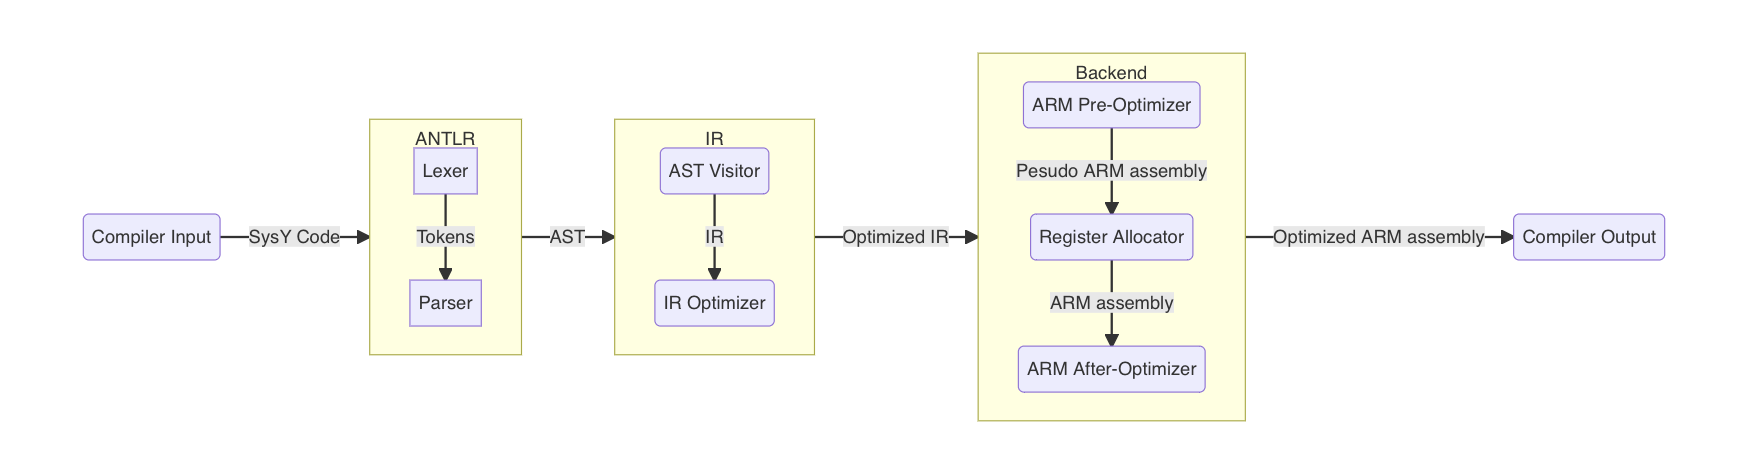
\includegraphics[width=\textwidth]{arch.png}
		\end{frame}
			
	\section{中端优化}
	
		\begin{frame}{SSA}
			\begin{itemize}
				\item SSA Construction: 构造 SSA,保证每个寄存器只有一次 Def
				\item SSA Destruction: 在中端优化的最后消除 $\Phi$ 指令
			\end{itemize}
		\end{frame}
		
		\begin{frame}{基本块优化}
			\begin{itemize}
				\item 消除不可达的基本块
				\item 消除分支条件可以推断为常量的分支
				\item 将基本块排列为正常顺序,使得同个循环内的代码是连续的若干个基本块,循环内的基本块按删去回边后 dfs 的逆后序排列
				\item 将无条件跳转的目标基本块的代码复制到跳转前的基本块,减少基本块个数
			\end{itemize}
		\end{frame}
		
		\begin{frame}{常规优化}
			\begin{itemize}
				\item Global Code Motion
				\item Global Value Numbering
				\item Dead Code Elimination: 消除无用指令 / 变量
				\item mem2reg: 全局变量转局部变量,局部变量放在寄存器上
			\end{itemize}
		\end{frame}
		
		\begin{frame}{过程间优化}
			\begin{itemize}
				\item Function Inline: 能 inline 的函数全部 inline,带递归的函数展开若干层
				\item 如果一个函数的某个参数在所有调用中相同,则将其替换为常量	
				\item 如果一个函数的返回值从未由调用者使用,则将返回值设为 0
				\item 尾递归转循环
			\end{itemize}
		\end{frame}
		
		\begin{frame}{副作用优化}
			\begin{itemize}
				\item 对不写内存的函数调用,分析读的内存是否发生改变,消除多余的调用
				\item 对于数组没有被修改过的情况,将对数组的固定下标的访问替换为数组全局初始化的值
				\item 如果局部变量的每个下标都只被赋值过一次,且赋值为常数,则将其提升为全局常量
				\item 将 main 函数开头的全局变量写操作吸收到全局变量初始化中
				\item 尽可能将读内存操作替换为上次读或写的值
				\item 如果写操作不会对之后的读操作产生影响,则删除写操作
			\end{itemize}
		\end{frame}
		
		\begin{frame}{循环变换}
			\begin{itemize}
				\item 对于循环次数固定且展开后指令数较小的循环,展开为顺序执行
				\item 对于循环次数不固定的循环,进行循环展开
				\item 消除 Reduction Variable
			\end{itemize}
		\end{frame}
		
		\begin{frame}{SIMD 与多线程}
			
		\end{frame}
	
	\section{后端优化}
	
		\begin{frame}{常规优化}
			\begin{itemize}
				\item Dead Code Elimination
				\item 对只含一条跳转指令的基本块,尽可能删除,但保证不出现基本块间的多重边
				\item 对只有一个前驱的基本块,将指令移动到前驱
				\item 分支指令转为条件执行
			\end{itemize}
		\end{frame}
		
		\begin{frame}{指令合并}
			
		\end{frame}
		
		\begin{frame}{寄存器分配}
			
		\end{frame}
	
\end{document}